% %% %%%%%%%%%%%%%%%%%%%%%%%%%%%%%%%%%%%%%%%%%%%%%%%%%%%%%%%%%%
% practica.tex
%
% Author:  Mauricio Matamoros
% License: MIT
%
% %% %%%%%%%%%%%%%%%%%%%%%%%%%%%%%%%%%%%%%%%%%%%%%%%%%%%%%%%%%%

% TEX-ROOT=references.bib
% CHKTEX-FILE 1
% CHKTEX-FILE 13
% CHKTEX-FILE 46
\documentclass[letterpaper,10.5pt]{article}
% %% %%%%%%%%%%%%%%%%%%%%%%%%%%%%%%%%%%%%%%%%%%%%%%%%%%%%%%%%%
%
% packages.tex
%
%  Author: Mauricio Matamoros
%  Date:   2020.02.28
%
%  Contiene la lista de paquetes requeridos para generar
%  el archivo-reporte de las prácticas de laboratorio
%
% %% %%%%%%%%%%%%%%%%%%%%%%%%%%%%%%%%%%%%%%%%%%%%%%%%%%%%%%%%%
% Archivo principal de LaTeX
%!TEX root = ../reporte.tex

\usepackage[utf8]{inputenc}                  % Soporte para utf8
\usepackage[T1]{fontenc}                     % Soporte extendido de caracteres unicode
\usepackage[english,spanish,mexico]{babel}   % Define el idioma del documento a español (México) con soporte para inglés
% Standard packages
\usepackage{float}                           % Imágenes flotantes en el documento
\usepackage{ifthen}                          % Soporte if-then en macros
\usepackage{xspace}                          % Soporte de autoespaciado en macros
\usepackage{xstring}                         % Operaciones con cadenas en macros
\usepackage{wrapfig}                         % Permite colocar texto al rededor de figuras y otros flotantes
\usepackage{booktabs}                        % Embellece tablas
\usepackage{csquotes}                        % Entrecomillado automático y manejo de citas textuales
\usepackage{fancyhdr}                        % Permite reconfigurar encabezado y pie de página
\usepackage{fancyvrb}                        % Define estilos para entornos Verbatim
\usepackage{geometry}                        % Permite reconfigurar la geometría del documento
\usepackage{graphicx}                        % Permite insertar imágenes en varios formatos
\usepackage{lastpage}                        % Referencia a la última página del documento
\usepackage{listings}                        % Define estilos para entornos de código de programación (sintaxis)
\usepackage{multicol}                        % Manejo de texto en varias columnas
\usepackage{tabularx}                        % Tablas con ancho de columna variable
\usepackage{algorithm}                       % Entorno para escribir algoritmos
\usepackage{algpseudocode}                   % Entorno para escribir algoritmos en pseudocódigo
\usepackage[justification=centering]{subcaption} % Permite imágenes en viñetas
\usepackage[all]{nowidow}                    % Control de viudas y huérfanas
\usepackage[inline]{enumitem}                % Añade opciones de configuración a listas
\usepackage[usenames,dvipsnames]{xcolor}     % Permite el uso de colores en el documento
% Referencing
\usepackage{varioref}                        % Gestión de referencias variables
\usepackage{hyperref}                        % Gestión de referencias e hipervínculos
\usepackage[noabbrev,nameinlink,spanish]{cleveref} % Gestión de referencias cruzadas inteligentes con hipervínculos
\usepackage[square, comma, numbers, sort&compress]{natbib} % Gestión de referencias bibliográficas


\newcommand{\lpar}{(}\newcommand{\rpar}{)} %CHKTEX 9
\newcommand{\IIC}{I\textsuperscript{2}C\xspace}
\newcommand{\GND}{\textsc{Gnd}\xspace}
\newcommand{\VCC}{\textsc{Vcc}\xspace}
\newcommand{\VDD}{\textsc{Vdd}\xspace}
\newcommand{\textbi}[1]{\textbf{\textit{#1}}}
\newcommand{\degreesC}[1]{%
	#1\textsuperscript{o}C\xspace{}%
}
\newcommand{\degreesF}[1]{%
	#1\textsuperscript{o}F\xspace{}%
}

% \newcommand{\VCC}{V\textsubscript{CC}\xspace{}}
% \newcommand{\GND}{\textsc{Gnd}\xspace{}}
% CHKTEX-FILE 26
% CHKTEX-FILE 36

\tcbuselibrary{most}
% \tcbuselibrary{listings,breakable}
% \usetikzlibrary{shadings,shadows}
% \usetikzlibrary{decorations.pathmorphing}
% \usetikzlibrary{patterns}
% \usetikzlibrary{spy}
% \usetikzlibrary{arrows.meta}

\newtcolorbox{importantbox}[1]{%
	enhanced,
	colback=red!5!white,%
	colframe=red!75!black,%
	fonttitle=\bfseries,%
	center title,
	title={#1},%
	drop fuzzy shadow
}


\newtcolorbox{greenbox}[1]{%
	enhanced,
	colback=Green!5!white,%
	colframe=Green!75!black,%
	fonttitle=\bfseries,%
	center title,
	title={#1},%
	drop fuzzy shadow
}

\newtcolorbox{marker}[1][]{%
	enhanced,
	before skip=2mm,after skip=3mm,
	boxrule=0.4pt,left=5mm,right=2mm,top=1mm,bottom=1mm,
	colback=yellow!50,
	colframe=yellow!20!black,
	sharp corners,rounded corners=southeast,arc is angular,arc=3mm,
%	underlay={%
%		\path[fill=tcbcolback!80!black] ([yshift=3mm]interior.south east)--++(-0.4,-0.1)--++(0.1,-0.2);
%		\path[draw=tcbcolframe,shorten <=-0.05mm,shorten >=-0.05mm] ([yshift=3mm]interior.south east)--++(-0.4,-0.1)--++(0.1,-0.2);
%		\path[fill=yellow!50!black,draw=none] (interior.south west) rectangle node[white]{\Huge\bfseries !} ([xshift=4mm]interior.north west);
%	},
	drop fuzzy shadow,#1
}

%CHKTEX-FILE 1
%CHKTEX-FILE 7
%CHKTEX-FILE 9
% Default fixed font does not support bold face
\DeclareFixedFont{\ttb}{T1}{txtt}{bx}{n}{8} % for bold
\DeclareFixedFont{\ttm}{T1}{txtt}{m}{n}{8}  % for normal

% Custom colors
\usepackage{color}
\definecolor{keywordsColor}{rgb}{0,0,0.5}
\definecolor{customColor}{rgb}{0.6,0,0}
\definecolor{stringColor}{rgb}{0,0.5,0}

% Code highlighting python
\renewcommand{\ttdefault}{pcr}
\lstset{
	language=Python,                              % the language of the code (can be overrided per snippet)
	backgroundcolor=\color{white},                % choose the background color
	basicstyle=\footnotesize\ttfamily,            % the size of the fonts that are used for the code
	breakatwhitespace=false,                      % sets if automatic breaks should only happen at whitespace
	breaklines=true,                              % sets automatic line breaking
	captionpos=t,                                 % sets the caption-position to bottom
	commentstyle=\color{gray},                    % comment style
	deletekeywords={},                            % if you want to delete keywords from the given language
%	escapeinside={\%*}{*)},                       % if you want to add LaTeX within your code
	extendedchars=true,                           % lets you use non-ASCII characters; for 8-bits encodings only, does not work with UTF-8
	frame=tb,                                     % adds a frame around the code
	keepspaces=true,                              % keeps spaces in text, useful for keeping indentation of code (possibly needs columns=flexible)
	keywordstyle=\color{keywordsColor}\bfseries,  % keyword style
	numbers=left,                                 % where to put the line-numbers; possible values are (none, left, right)
	numbersep=5pt,                                % how far the line-numbers are from the code
	numberstyle=\tiny\color{gray},                % the style that is used for the line-numbers
	rulecolor=\color{black},                      % if not set, the frame-color may be changed on line-breaks within not-black text (e.g. comments (green here))
	showspaces=false,                             % show spaces everywhere adding particular underscores; it overrides 'showstringspaces'
	showstringspaces=false,                       % underline spaces within strings only
	showtabs=false,                               % show tabs within strings adding particular underscores
	stepnumber=1,                                 % the step between two line-numbers. If it's 1, each line will be numbered
	stringstyle=\color{stringColor},              % string literal style
	tabsize=2,                                    % sets default tabsize to 2 spaces
	title=\lstname,                               % show the filename of files included with \lstinputlisting; also try caption instead of title
	columns=fixed,                                % Using fixed column width (for e.g. nice alignment)
	otherkeywords={self},                         % if you want to add more keywords to the set
	emphstyle=\color{customColor}\bfseries,       % Custom highlighting style
	emph={__init__,__main__,True,False,None},     % Custom highlighting keywords
	xleftmargin=1cm,                              % Left margin
	xrightmargin=1cm,                             % Right margin
	% Unicode compatibility
	inputencoding=utf8,
	literate={%
	            {Á}{{\'a}}1 {É}{{\'E}}1 {Í}{{\'I}}1 {Ó}{{\'O}}1 {Ú}{{\'U}}1%
	            {á}{{\'a}}1 {é}{{\'e}}1 {í}{{\'i}}1 {ó}{{\'o}}1 {ú}{{\'u}}1%
	            {À}{{\`A}}1 {È}{{\'E}}1 {Ì}{{\`I}}1 {Ò}{{\`O}}1 {Ù}{{\`U}}1%
	            {à}{{\`a}}1 {è}{{\`e}}1 {ì}{{\`i}}1 {ò}{{\`o}}1 {ù}{{\`u}}1%
	            {Ä}{{\"A}}1 {Ë}{{\"E}}1 {Ï}{{\"I}}1 {Ö}{{\"O}}1 {Ü}{{\"U}}1%
	            {ä}{{\"a}}1 {ë}{{\"e}}1 {ï}{{\"i}}1 {ö}{{\"o}}1 {ü}{{\"u}}1%
	            {Â}{{\^A}}1 {Ê}{{\^E}}1 {Î}{{\^I}}1 {Ô}{{\^O}}1 {Û}{{\^U}}1%
	            {â}{{\^a}}1 {ê}{{\^e}}1 {î}{{\^i}}1 {ô}{{\^o}}1 {û}{{\^u}}1% CHKTEX 19
	            {Ã}{{\~a}}1 {Ẽ}{{\~E}}1 {Ĩ}{{\~I}}1 {Õ}{{\~O}}1 {Ũ}{{\~U}}1 {Ñ}{{\~N}}1%
	            {ã}{{\~a}}1 {ẽ}{{\~e}}1 {ĩ}{{\~i}}1 {õ}{{\~o}}1 {ũ}{{\~u}}1 {ñ}{{\~n}}1%
	            {œ}{{\oe}}1 {Œ}{{\OE}}1 {æ}{{\ae}}1 {Æ}{{\AE}}1 {ß}{{\ss}}1%
	            {ç}{{\c c}}1 {Ç}{{\c C}}1 {ø}{{\o}}1 {å}{{\r a}}1 {Å}{{\r A}}1%
	            {€}{{\EUR}}1 {£}{{\pounds}}1 {×}{{\(\times\)}}1% CHKTEX 21
	            {°}{{\textsuperscript{o}}}1%
	            {¹}{{\textsuperscript{1}}}1%
	            {²}{{\textsuperscript{2}}}1%
	            {³}{{\textsuperscript{3}}}1%
	            {⁴}{{\textsuperscript{4}}}1% CHKTEX 19
	            {⁵}{{\textsuperscript{5}}}1% CHKTEX 19
	            {⁶}{{\textsuperscript{6}}}1% CHKTEX 19
	            {⁷}{{\textsuperscript{7}}}1% CHKTEX 19
	            {⁸}{{\textsuperscript{8}}}1% CHKTEX 19
	            {⁹}{{\textsuperscript{9}}}1% CHKTEX 19
	            {⁰}{{\textsuperscript{0}}}1% CHKTEX 19
%	            {A}{{\textAlpha}}1
	            {α}{{\textalpha}}1%
%	            {B}{{\textBeta}}1
	            {β}{{\textbeta}}1%
	            {Γ}{{\textGamma}}1
	            {γ}{{\textgamma}}1%
	            {Δ}{{\textDelta}}1
	            {δ}{{\textdelta}}1% CHKTEX 19
%	            {E}{{\textEpsilon}}1
	            {ϵ}{{\textepsilon}}1%
%	            {Z}{{\textZeta}}1
	            {ζ}{{\textzeta}}1%
%	            {H}{{\textEta}}1
	            {η}{{\texteta}}1%
	            {Θ}{{\textTheta}}1
	            {θ}{{\texttheta}}1%
%	            {I}{{\textIota}}1
	            {ι}{{\textiota}}1%
%	            {K}{{\textKappa}}1
	            {κ}{{\textkappa}}1%
	            {Λ}{{\textLambda}}1
	            {λ}{{\textlambda}}1%
%	            {M}{{\textMu}}1
	            {μ}{{\textmu}}1%
%	            {N}{{\textNu}}1
	            {ν}{{\textnu}}1%
	            {Ξ}{{\textXi}}1
	            {ξ}{{\textxi}}1%
%	            {O}{{\textOmikron}}1
%	            {o}{{\textomikron}}1%
	            {Π}{{\textPi}}1
	            {π}{{\textpi}}1%
%	            {P}{{\textRho}}1
	            {ρ}{{\textrho}}1%
	            {Σ}{{\textSigma}}1
	            {σ}{{\textsigma}}1%
%	            {T}{{\textTau}}1
	            {τ}{{\texttau}}1%
	            {ϒ}{{\textUpsilon}}1
	            {υ}{{\textupsilon}}1%
	            {Φ}{{\textPhi}}1
	            {ϕ}{{\textphi}}1%
%	            {X}{{\textChi}}1
	            {χ}{{\textchi}}1%
	            {Ψ}{{\textPsi}}1
	            {ψ}{{\textpsi}}1%
	            {Ω}{{\textOmega}}1
	            {ω}{{\textomega}}1%
	            {ζ}{{\varsigma}}1%
%	            {}{{\straightphi}}1%
%	            {}{{\scripttheta}}1%
%	            {}{{\straighttheta}}1%
%	            {}{{\straightepsilon}}1%
	         },
}

\lstdefinestyle{c_with_comments}%
{
	language     = c,
	morecomment  = [l]{//},
	morecomment  = [s]{/*}{*/},
	breaklines,
}

\lstdefinestyle{c_without_comments}{%
	style        = c_with_comments,
	% numbers      = none,
	% keepspaces   = false,
	morecomment  = [l][\nullfont]{//},
	morecomment  = [is]{//}{\^^M},
	morecomment  = [is]{/*}{*/},
	emptylines   = *1,
}

\lstdefinestyle{py_without_comments}{%
	language     = python,
	morecomment  = [l][\nullfont]{\#},
	% morecomment  = [il]{\#},
	% morecomment  = [is]{\#}{\^^M},
	emptylines   = *1,
}

\lstdefinestyle{py_without_doclines}{%
	morecomment  = [is]{'''}{'''},%CHKTEX 23
	morecomment  = [is]{"""}{"""},%CHKTEX 18
	morecomment  = [is]{\#'''}{'''},%CHKTEX 23
	morecomment  = [is]{\#"""}{"""},%CHKTEX 18
}

\lstdefinelanguage{conf}
{
	basicstyle=\ttfamily\small,
	columns=fullflexible,
	morecomment=[s][\color{Orchid}\bfseries]{[}{]},
	morecomment=[l]{\#},
	morecomment=[l]{;},
	commentstyle=\color{gray}\ttfamily,
	% morekeywords={},
	% otherkeywords={=,:},
	% keywordstyle={\color{Green}\bfseries}
}

% \captionsetup[lstlisting]{font={small,tt}}
\captionsetup[lstlisting]{%
	font={small},
}



\DefineVerbatimEnvironment{Verbatim}{Verbatim}{%
	fontsize=\footnotesize,%
	frame=leftline,%
	framesep=2em,    % separation between frame and text
}

\RecustomVerbatimCommand{\VerbatimInput}{VerbatimInput}{%
	fontsize=\footnotesize,
%	frame=lines,            % top and bottom rule only
	frame=leftline,         % left rule only
	numbers=left,           % Line numbers on the left
	numbersep=0.25em,       % Gap between numbers and verbatim lines
	xleftmargin=4em,        % Indentation to add at the start of each line
	xrightmargin=4em,       % Right margin to add after each line
	framesep=0.5em,         % separation between frame and text
	rulecolor=\color{Gray}, % Color of the lines
	labelposition=topline,  %
	samepage=false,         % When true, prevents verbatim environment from
	                        % being broken between pages
%	commandchars=\|\(\),    % escape character and argument delimiters for
	                        % commands within the verbatim
%	commentchar=*           % comment character
}


% CHKTEX-FILE 1
% CHKTEX-FILE 13
% CHKTEX-FILE 18
% CHKTEX-FILE 35
\documentclass[letterpaper,12pt,twocolumn]{article}
% Input encodign

% %% %%%%%%%%%%%%%%%%%%%%%%%%%%%%%%%%%%%%%%%%%%%%%%%%%%%%%%%%%
%
% packages.tex
%
%  Author: Mauricio Matamoros
%  Date:   2020.02.28
%
%  Contiene la lista de paquetes requeridos para generar
%  el archivo-reporte de las prácticas de laboratorio
%
% %% %%%%%%%%%%%%%%%%%%%%%%%%%%%%%%%%%%%%%%%%%%%%%%%%%%%%%%%%%
% Archivo principal de LaTeX
%!TEX root = ../reporte.tex

\usepackage[utf8]{inputenc}                  % Soporte para utf8
\usepackage[T1]{fontenc}                     % Soporte extendido de caracteres unicode
\usepackage[english,spanish,mexico]{babel}   % Define el idioma del documento a español (México) con soporte para inglés
% Standard packages
\usepackage{float}                           % Imágenes flotantes en el documento
\usepackage{ifthen}                          % Soporte if-then en macros
\usepackage{xspace}                          % Soporte de autoespaciado en macros
\usepackage{xstring}                         % Operaciones con cadenas en macros
\usepackage{wrapfig}                         % Permite colocar texto al rededor de figuras y otros flotantes
\usepackage{booktabs}                        % Embellece tablas
\usepackage{csquotes}                        % Entrecomillado automático y manejo de citas textuales
\usepackage{fancyhdr}                        % Permite reconfigurar encabezado y pie de página
\usepackage{fancyvrb}                        % Define estilos para entornos Verbatim
\usepackage{geometry}                        % Permite reconfigurar la geometría del documento
\usepackage{graphicx}                        % Permite insertar imágenes en varios formatos
\usepackage{lastpage}                        % Referencia a la última página del documento
\usepackage{listings}                        % Define estilos para entornos de código de programación (sintaxis)
\usepackage{multicol}                        % Manejo de texto en varias columnas
\usepackage{tabularx}                        % Tablas con ancho de columna variable
\usepackage{algorithm}                       % Entorno para escribir algoritmos
\usepackage{algpseudocode}                   % Entorno para escribir algoritmos en pseudocódigo
\usepackage[justification=centering]{subcaption} % Permite imágenes en viñetas
\usepackage[all]{nowidow}                    % Control de viudas y huérfanas
\usepackage[inline]{enumitem}                % Añade opciones de configuración a listas
\usepackage[usenames,dvipsnames]{xcolor}     % Permite el uso de colores en el documento
% Referencing
\usepackage{varioref}                        % Gestión de referencias variables
\usepackage{hyperref}                        % Gestión de referencias e hipervínculos
\usepackage[noabbrev,nameinlink,spanish]{cleveref} % Gestión de referencias cruzadas inteligentes con hipervínculos
\usepackage[square, comma, numbers, sort&compress]{natbib} % Gestión de referencias bibliográficas


\newcommand{\lpar}{(}\newcommand{\rpar}{)} %CHKTEX 9
\newcommand{\IIC}{I\textsuperscript{2}C\xspace}
\newcommand{\GND}{\textsc{Gnd}\xspace}
\newcommand{\VCC}{\textsc{Vcc}\xspace}
\newcommand{\VDD}{\textsc{Vdd}\xspace}
\newcommand{\textbi}[1]{\textbf{\textit{#1}}}
\newcommand{\degreesC}[1]{%
	#1\textsuperscript{o}C\xspace{}%
}
\newcommand{\degreesF}[1]{%
	#1\textsuperscript{o}F\xspace{}%
}

% \newcommand{\VCC}{V\textsubscript{CC}\xspace{}}
% \newcommand{\GND}{\textsc{Gnd}\xspace{}}
% CHKTEX-FILE 1
% CHKTEX-FILE 13
% CHKTEX-FILE 18
% CHKTEX-FILE 35
\documentclass[letterpaper,12pt,twocolumn]{article}
% Input encodign

% %% %%%%%%%%%%%%%%%%%%%%%%%%%%%%%%%%%%%%%%%%%%%%%%%%%%%%%%%%%
%
% packages.tex
%
%  Author: Mauricio Matamoros
%  Date:   2020.02.28
%
%  Contiene la lista de paquetes requeridos para generar
%  el archivo-reporte de las prácticas de laboratorio
%
% %% %%%%%%%%%%%%%%%%%%%%%%%%%%%%%%%%%%%%%%%%%%%%%%%%%%%%%%%%%
% Archivo principal de LaTeX
%!TEX root = ../reporte.tex

\usepackage[utf8]{inputenc}                  % Soporte para utf8
\usepackage[T1]{fontenc}                     % Soporte extendido de caracteres unicode
\usepackage[english,spanish,mexico]{babel}   % Define el idioma del documento a español (México) con soporte para inglés
% Standard packages
\usepackage{float}                           % Imágenes flotantes en el documento
\usepackage{ifthen}                          % Soporte if-then en macros
\usepackage{xspace}                          % Soporte de autoespaciado en macros
\usepackage{xstring}                         % Operaciones con cadenas en macros
\usepackage{wrapfig}                         % Permite colocar texto al rededor de figuras y otros flotantes
\usepackage{booktabs}                        % Embellece tablas
\usepackage{csquotes}                        % Entrecomillado automático y manejo de citas textuales
\usepackage{fancyhdr}                        % Permite reconfigurar encabezado y pie de página
\usepackage{fancyvrb}                        % Define estilos para entornos Verbatim
\usepackage{geometry}                        % Permite reconfigurar la geometría del documento
\usepackage{graphicx}                        % Permite insertar imágenes en varios formatos
\usepackage{lastpage}                        % Referencia a la última página del documento
\usepackage{listings}                        % Define estilos para entornos de código de programación (sintaxis)
\usepackage{multicol}                        % Manejo de texto en varias columnas
\usepackage{tabularx}                        % Tablas con ancho de columna variable
\usepackage{algorithm}                       % Entorno para escribir algoritmos
\usepackage{algpseudocode}                   % Entorno para escribir algoritmos en pseudocódigo
\usepackage[justification=centering]{subcaption} % Permite imágenes en viñetas
\usepackage[all]{nowidow}                    % Control de viudas y huérfanas
\usepackage[inline]{enumitem}                % Añade opciones de configuración a listas
\usepackage[usenames,dvipsnames]{xcolor}     % Permite el uso de colores en el documento
% Referencing
\usepackage{varioref}                        % Gestión de referencias variables
\usepackage{hyperref}                        % Gestión de referencias e hipervínculos
\usepackage[noabbrev,nameinlink,spanish]{cleveref} % Gestión de referencias cruzadas inteligentes con hipervínculos
\usepackage[square, comma, numbers, sort&compress]{natbib} % Gestión de referencias bibliográficas


\newcommand{\lpar}{(}\newcommand{\rpar}{)} %CHKTEX 9
\newcommand{\IIC}{I\textsuperscript{2}C\xspace}
\newcommand{\GND}{\textsc{Gnd}\xspace}
\newcommand{\VCC}{\textsc{Vcc}\xspace}
\newcommand{\VDD}{\textsc{Vdd}\xspace}
\newcommand{\textbi}[1]{\textbf{\textit{#1}}}
\newcommand{\degreesC}[1]{%
	#1\textsuperscript{o}C\xspace{}%
}
\newcommand{\degreesF}[1]{%
	#1\textsuperscript{o}F\xspace{}%
}

% \newcommand{\VCC}{V\textsubscript{CC}\xspace{}}
% \newcommand{\GND}{\textsc{Gnd}\xspace{}}
% CHKTEX-FILE 1
% CHKTEX-FILE 13
% CHKTEX-FILE 18
% CHKTEX-FILE 35
\documentclass[letterpaper,12pt,twocolumn]{article}
% Input encodign

\input{setup/packages}
\input{setup/macros}
\input{setup/document}
\input{setup/listings}

\author{\footnotesize Autor: José Mauricio Matamoros de Maria y Campos}
\title{Especificación para reportes de lectura}
\date{}


% Document body
\begin{document}
\maketitle

\section*{Reportes de lectura}
El objetivo de las lecturas asignadas como tarea es fomentar en el alumno el hábito de la lectura, tanto de documentos técnicos como literarios, ya sean estos en español o en inglés, además de incrementar las habilidades de comprensión de lectura, concreción de ideas, síntesis y redacción de texto en prosa.

Leer es muy importante en el aprendizaje pues la mayor parte de lo que se aprende se hace por medio de la lectura.
Cuando se quiere aprender algo, lo primero que se hace es leer.

Cuando se lee un texto con fines de estudio se resaltan las ideas importantes, se resume, se separan las ideas principales y se formulan cuestionarios para mejor comprender el texto. Cuando se lee por entretenimiento (por ejemplo un cuento o una novela), el texto se analiza y se relacionan hechos y situaciones a fin de poder disfrutar de él.

Un reporte de lectura es un informe escrito acerca del texto que se leyó.
Este informe debe contener los siguientes datos:

\begin{itemize}[noitemsep]
	\item Título del texto y nombre del autor
	\item Tema o asunto que trata
	\item Resumen, síntesis o reseña del texto
	\item Análisis crítico del contenido del texto
	\item Opinión personal del contenido de la lectura
	\item Conclusiones de la lectura
\end{itemize}

En el caso de texto literario no se espera un resumen, síntesis o reseña del texto, sino que deberá comentarse sobre la temática del mismo y resaltar los puntos más importantes, dejando claras sus impresiones y comentarios sobre el texto.

Tome en cuenta que ni la síntesis ni los resúmenes implican copiar y pegar párrafos enteros del texto. Lo importante es distinguir las ideas principales, hacerlas propias y (salvo que sean definiciones), parafrasearlas, es decir,  expresarlas en sus propias palabras.

Pasos para elaborar un reporte de lectura
\begin{enumerate}[noitemsep]
	\item Lea atentamente el texto. Evite distractores como música fuerte, televisión, teléfono, etc.
	\item Anote los términos y palabras que no conozca o entienda e investigue su significado en un diccionario.
	\item Una vez aclarados los términos desconocidos y palabras nuevas, vuelva a leer el texto para comprenderlo mejor.
	\item En la segunda lectura subraye o marque las ideas principales del texto.
	%Procure no escribir en los libros, especialmente si no le pertenecen. Si desea hacer anotaciones, utilice un lápiz blando y escriba con suavidad, o de preferencia use fotocopias.
	\item Tome las ideas principales, abstraígalas, analícelas y sólo entonces redacte su escrito.
\end{enumerate}
\end{document}

%CHKTEX-FILE 1
%CHKTEX-FILE 7
%CHKTEX-FILE 9
% Default fixed font does not support bold face
\DeclareFixedFont{\ttb}{T1}{txtt}{bx}{n}{8} % for bold
\DeclareFixedFont{\ttm}{T1}{txtt}{m}{n}{8}  % for normal

% Custom colors
\usepackage{color}
\definecolor{keywordsColor}{rgb}{0,0,0.5}
\definecolor{customColor}{rgb}{0.6,0,0}
\definecolor{stringColor}{rgb}{0,0.5,0}

% Code highlighting python
\renewcommand{\ttdefault}{pcr}
\lstset{
	language=Python,                              % the language of the code (can be overrided per snippet)
	backgroundcolor=\color{white},                % choose the background color
	basicstyle=\footnotesize\ttfamily,            % the size of the fonts that are used for the code
	breakatwhitespace=false,                      % sets if automatic breaks should only happen at whitespace
	breaklines=true,                              % sets automatic line breaking
	captionpos=t,                                 % sets the caption-position to bottom
	commentstyle=\color{gray},                    % comment style
	deletekeywords={},                            % if you want to delete keywords from the given language
%	escapeinside={\%*}{*)},                       % if you want to add LaTeX within your code
	extendedchars=true,                           % lets you use non-ASCII characters; for 8-bits encodings only, does not work with UTF-8
	frame=tb,                                     % adds a frame around the code
	keepspaces=true,                              % keeps spaces in text, useful for keeping indentation of code (possibly needs columns=flexible)
	keywordstyle=\color{keywordsColor}\bfseries,  % keyword style
	numbers=left,                                 % where to put the line-numbers; possible values are (none, left, right)
	numbersep=5pt,                                % how far the line-numbers are from the code
	numberstyle=\tiny\color{gray},                % the style that is used for the line-numbers
	rulecolor=\color{black},                      % if not set, the frame-color may be changed on line-breaks within not-black text (e.g. comments (green here))
	showspaces=false,                             % show spaces everywhere adding particular underscores; it overrides 'showstringspaces'
	showstringspaces=false,                       % underline spaces within strings only
	showtabs=false,                               % show tabs within strings adding particular underscores
	stepnumber=1,                                 % the step between two line-numbers. If it's 1, each line will be numbered
	stringstyle=\color{stringColor},              % string literal style
	tabsize=2,                                    % sets default tabsize to 2 spaces
	title=\lstname,                               % show the filename of files included with \lstinputlisting; also try caption instead of title
	columns=fixed,                                % Using fixed column width (for e.g. nice alignment)
	otherkeywords={self},                         % if you want to add more keywords to the set
	emphstyle=\color{customColor}\bfseries,       % Custom highlighting style
	emph={__init__,__main__,True,False,None},     % Custom highlighting keywords
	xleftmargin=1cm,                              % Left margin
	xrightmargin=1cm,                             % Right margin
	% Unicode compatibility
	inputencoding=utf8,
	literate={%
	            {Á}{{\'a}}1 {É}{{\'E}}1 {Í}{{\'I}}1 {Ó}{{\'O}}1 {Ú}{{\'U}}1%
	            {á}{{\'a}}1 {é}{{\'e}}1 {í}{{\'i}}1 {ó}{{\'o}}1 {ú}{{\'u}}1%
	            {À}{{\`A}}1 {È}{{\'E}}1 {Ì}{{\`I}}1 {Ò}{{\`O}}1 {Ù}{{\`U}}1%
	            {à}{{\`a}}1 {è}{{\`e}}1 {ì}{{\`i}}1 {ò}{{\`o}}1 {ù}{{\`u}}1%
	            {Ä}{{\"A}}1 {Ë}{{\"E}}1 {Ï}{{\"I}}1 {Ö}{{\"O}}1 {Ü}{{\"U}}1%
	            {ä}{{\"a}}1 {ë}{{\"e}}1 {ï}{{\"i}}1 {ö}{{\"o}}1 {ü}{{\"u}}1%
	            {Â}{{\^A}}1 {Ê}{{\^E}}1 {Î}{{\^I}}1 {Ô}{{\^O}}1 {Û}{{\^U}}1%
	            {â}{{\^a}}1 {ê}{{\^e}}1 {î}{{\^i}}1 {ô}{{\^o}}1 {û}{{\^u}}1% CHKTEX 19
	            {Ã}{{\~a}}1 {Ẽ}{{\~E}}1 {Ĩ}{{\~I}}1 {Õ}{{\~O}}1 {Ũ}{{\~U}}1 {Ñ}{{\~N}}1%
	            {ã}{{\~a}}1 {ẽ}{{\~e}}1 {ĩ}{{\~i}}1 {õ}{{\~o}}1 {ũ}{{\~u}}1 {ñ}{{\~n}}1%
	            {œ}{{\oe}}1 {Œ}{{\OE}}1 {æ}{{\ae}}1 {Æ}{{\AE}}1 {ß}{{\ss}}1%
	            {ç}{{\c c}}1 {Ç}{{\c C}}1 {ø}{{\o}}1 {å}{{\r a}}1 {Å}{{\r A}}1%
	            {€}{{\EUR}}1 {£}{{\pounds}}1 {×}{{\(\times\)}}1% CHKTEX 21
	            {°}{{\textsuperscript{o}}}1%
	            {¹}{{\textsuperscript{1}}}1%
	            {²}{{\textsuperscript{2}}}1%
	            {³}{{\textsuperscript{3}}}1%
	            {⁴}{{\textsuperscript{4}}}1% CHKTEX 19
	            {⁵}{{\textsuperscript{5}}}1% CHKTEX 19
	            {⁶}{{\textsuperscript{6}}}1% CHKTEX 19
	            {⁷}{{\textsuperscript{7}}}1% CHKTEX 19
	            {⁸}{{\textsuperscript{8}}}1% CHKTEX 19
	            {⁹}{{\textsuperscript{9}}}1% CHKTEX 19
	            {⁰}{{\textsuperscript{0}}}1% CHKTEX 19
%	            {A}{{\textAlpha}}1
	            {α}{{\textalpha}}1%
%	            {B}{{\textBeta}}1
	            {β}{{\textbeta}}1%
	            {Γ}{{\textGamma}}1
	            {γ}{{\textgamma}}1%
	            {Δ}{{\textDelta}}1
	            {δ}{{\textdelta}}1% CHKTEX 19
%	            {E}{{\textEpsilon}}1
	            {ϵ}{{\textepsilon}}1%
%	            {Z}{{\textZeta}}1
	            {ζ}{{\textzeta}}1%
%	            {H}{{\textEta}}1
	            {η}{{\texteta}}1%
	            {Θ}{{\textTheta}}1
	            {θ}{{\texttheta}}1%
%	            {I}{{\textIota}}1
	            {ι}{{\textiota}}1%
%	            {K}{{\textKappa}}1
	            {κ}{{\textkappa}}1%
	            {Λ}{{\textLambda}}1
	            {λ}{{\textlambda}}1%
%	            {M}{{\textMu}}1
	            {μ}{{\textmu}}1%
%	            {N}{{\textNu}}1
	            {ν}{{\textnu}}1%
	            {Ξ}{{\textXi}}1
	            {ξ}{{\textxi}}1%
%	            {O}{{\textOmikron}}1
%	            {o}{{\textomikron}}1%
	            {Π}{{\textPi}}1
	            {π}{{\textpi}}1%
%	            {P}{{\textRho}}1
	            {ρ}{{\textrho}}1%
	            {Σ}{{\textSigma}}1
	            {σ}{{\textsigma}}1%
%	            {T}{{\textTau}}1
	            {τ}{{\texttau}}1%
	            {ϒ}{{\textUpsilon}}1
	            {υ}{{\textupsilon}}1%
	            {Φ}{{\textPhi}}1
	            {ϕ}{{\textphi}}1%
%	            {X}{{\textChi}}1
	            {χ}{{\textchi}}1%
	            {Ψ}{{\textPsi}}1
	            {ψ}{{\textpsi}}1%
	            {Ω}{{\textOmega}}1
	            {ω}{{\textomega}}1%
	            {ζ}{{\varsigma}}1%
%	            {}{{\straightphi}}1%
%	            {}{{\scripttheta}}1%
%	            {}{{\straighttheta}}1%
%	            {}{{\straightepsilon}}1%
	         },
}

\lstdefinestyle{c_with_comments}%
{
	language     = c,
	morecomment  = [l]{//},
	morecomment  = [s]{/*}{*/},
	breaklines,
}

\lstdefinestyle{c_without_comments}{%
	style        = c_with_comments,
	% numbers      = none,
	% keepspaces   = false,
	morecomment  = [l][\nullfont]{//},
	morecomment  = [is]{//}{\^^M},
	morecomment  = [is]{/*}{*/},
	emptylines   = *1,
}

\lstdefinestyle{py_without_comments}{%
	language     = python,
	morecomment  = [l][\nullfont]{\#},
	% morecomment  = [il]{\#},
	% morecomment  = [is]{\#}{\^^M},
	emptylines   = *1,
}

\lstdefinestyle{py_without_doclines}{%
	morecomment  = [is]{'''}{'''},%CHKTEX 23
	morecomment  = [is]{"""}{"""},%CHKTEX 18
	morecomment  = [is]{\#'''}{'''},%CHKTEX 23
	morecomment  = [is]{\#"""}{"""},%CHKTEX 18
}

\lstdefinelanguage{conf}
{
	basicstyle=\ttfamily\small,
	columns=fullflexible,
	morecomment=[s][\color{Orchid}\bfseries]{[}{]},
	morecomment=[l]{\#},
	morecomment=[l]{;},
	commentstyle=\color{gray}\ttfamily,
	% morekeywords={},
	% otherkeywords={=,:},
	% keywordstyle={\color{Green}\bfseries}
}

% \captionsetup[lstlisting]{font={small,tt}}
\captionsetup[lstlisting]{%
	font={small},
}



\DefineVerbatimEnvironment{Verbatim}{Verbatim}{%
	fontsize=\footnotesize,%
	frame=leftline,%
	framesep=2em,    % separation between frame and text
}

\RecustomVerbatimCommand{\VerbatimInput}{VerbatimInput}{%
	fontsize=\footnotesize,
%	frame=lines,            % top and bottom rule only
	frame=leftline,         % left rule only
	numbers=left,           % Line numbers on the left
	numbersep=0.25em,       % Gap between numbers and verbatim lines
	xleftmargin=4em,        % Indentation to add at the start of each line
	xrightmargin=4em,       % Right margin to add after each line
	framesep=0.5em,         % separation between frame and text
	rulecolor=\color{Gray}, % Color of the lines
	labelposition=topline,  %
	samepage=false,         % When true, prevents verbatim environment from
	                        % being broken between pages
%	commandchars=\|\(\),    % escape character and argument delimiters for
	                        % commands within the verbatim
%	commentchar=*           % comment character
}



\author{\footnotesize Autor: José Mauricio Matamoros de Maria y Campos}
\title{Especificación para reportes de lectura}
\date{}


% Document body
\begin{document}
\maketitle

\section*{Reportes de lectura}
El objetivo de las lecturas asignadas como tarea es fomentar en el alumno el hábito de la lectura, tanto de documentos técnicos como literarios, ya sean estos en español o en inglés, además de incrementar las habilidades de comprensión de lectura, concreción de ideas, síntesis y redacción de texto en prosa.

Leer es muy importante en el aprendizaje pues la mayor parte de lo que se aprende se hace por medio de la lectura.
Cuando se quiere aprender algo, lo primero que se hace es leer.

Cuando se lee un texto con fines de estudio se resaltan las ideas importantes, se resume, se separan las ideas principales y se formulan cuestionarios para mejor comprender el texto. Cuando se lee por entretenimiento (por ejemplo un cuento o una novela), el texto se analiza y se relacionan hechos y situaciones a fin de poder disfrutar de él.

Un reporte de lectura es un informe escrito acerca del texto que se leyó.
Este informe debe contener los siguientes datos:

\begin{itemize}[noitemsep]
	\item Título del texto y nombre del autor
	\item Tema o asunto que trata
	\item Resumen, síntesis o reseña del texto
	\item Análisis crítico del contenido del texto
	\item Opinión personal del contenido de la lectura
	\item Conclusiones de la lectura
\end{itemize}

En el caso de texto literario no se espera un resumen, síntesis o reseña del texto, sino que deberá comentarse sobre la temática del mismo y resaltar los puntos más importantes, dejando claras sus impresiones y comentarios sobre el texto.

Tome en cuenta que ni la síntesis ni los resúmenes implican copiar y pegar párrafos enteros del texto. Lo importante es distinguir las ideas principales, hacerlas propias y (salvo que sean definiciones), parafrasearlas, es decir,  expresarlas en sus propias palabras.

Pasos para elaborar un reporte de lectura
\begin{enumerate}[noitemsep]
	\item Lea atentamente el texto. Evite distractores como música fuerte, televisión, teléfono, etc.
	\item Anote los términos y palabras que no conozca o entienda e investigue su significado en un diccionario.
	\item Una vez aclarados los términos desconocidos y palabras nuevas, vuelva a leer el texto para comprenderlo mejor.
	\item En la segunda lectura subraye o marque las ideas principales del texto.
	%Procure no escribir en los libros, especialmente si no le pertenecen. Si desea hacer anotaciones, utilice un lápiz blando y escriba con suavidad, o de preferencia use fotocopias.
	\item Tome las ideas principales, abstraígalas, analícelas y sólo entonces redacte su escrito.
\end{enumerate}
\end{document}

%CHKTEX-FILE 1
%CHKTEX-FILE 7
%CHKTEX-FILE 9
% Default fixed font does not support bold face
\DeclareFixedFont{\ttb}{T1}{txtt}{bx}{n}{8} % for bold
\DeclareFixedFont{\ttm}{T1}{txtt}{m}{n}{8}  % for normal

% Custom colors
\usepackage{color}
\definecolor{keywordsColor}{rgb}{0,0,0.5}
\definecolor{customColor}{rgb}{0.6,0,0}
\definecolor{stringColor}{rgb}{0,0.5,0}

% Code highlighting python
\renewcommand{\ttdefault}{pcr}
\lstset{
	language=Python,                              % the language of the code (can be overrided per snippet)
	backgroundcolor=\color{white},                % choose the background color
	basicstyle=\footnotesize\ttfamily,            % the size of the fonts that are used for the code
	breakatwhitespace=false,                      % sets if automatic breaks should only happen at whitespace
	breaklines=true,                              % sets automatic line breaking
	captionpos=t,                                 % sets the caption-position to bottom
	commentstyle=\color{gray},                    % comment style
	deletekeywords={},                            % if you want to delete keywords from the given language
%	escapeinside={\%*}{*)},                       % if you want to add LaTeX within your code
	extendedchars=true,                           % lets you use non-ASCII characters; for 8-bits encodings only, does not work with UTF-8
	frame=tb,                                     % adds a frame around the code
	keepspaces=true,                              % keeps spaces in text, useful for keeping indentation of code (possibly needs columns=flexible)
	keywordstyle=\color{keywordsColor}\bfseries,  % keyword style
	numbers=left,                                 % where to put the line-numbers; possible values are (none, left, right)
	numbersep=5pt,                                % how far the line-numbers are from the code
	numberstyle=\tiny\color{gray},                % the style that is used for the line-numbers
	rulecolor=\color{black},                      % if not set, the frame-color may be changed on line-breaks within not-black text (e.g. comments (green here))
	showspaces=false,                             % show spaces everywhere adding particular underscores; it overrides 'showstringspaces'
	showstringspaces=false,                       % underline spaces within strings only
	showtabs=false,                               % show tabs within strings adding particular underscores
	stepnumber=1,                                 % the step between two line-numbers. If it's 1, each line will be numbered
	stringstyle=\color{stringColor},              % string literal style
	tabsize=2,                                    % sets default tabsize to 2 spaces
	title=\lstname,                               % show the filename of files included with \lstinputlisting; also try caption instead of title
	columns=fixed,                                % Using fixed column width (for e.g. nice alignment)
	otherkeywords={self},                         % if you want to add more keywords to the set
	emphstyle=\color{customColor}\bfseries,       % Custom highlighting style
	emph={__init__,__main__,True,False,None},     % Custom highlighting keywords
	xleftmargin=1cm,                              % Left margin
	xrightmargin=1cm,                             % Right margin
	% Unicode compatibility
	inputencoding=utf8,
	literate={%
	            {Á}{{\'a}}1 {É}{{\'E}}1 {Í}{{\'I}}1 {Ó}{{\'O}}1 {Ú}{{\'U}}1%
	            {á}{{\'a}}1 {é}{{\'e}}1 {í}{{\'i}}1 {ó}{{\'o}}1 {ú}{{\'u}}1%
	            {À}{{\`A}}1 {È}{{\'E}}1 {Ì}{{\`I}}1 {Ò}{{\`O}}1 {Ù}{{\`U}}1%
	            {à}{{\`a}}1 {è}{{\`e}}1 {ì}{{\`i}}1 {ò}{{\`o}}1 {ù}{{\`u}}1%
	            {Ä}{{\"A}}1 {Ë}{{\"E}}1 {Ï}{{\"I}}1 {Ö}{{\"O}}1 {Ü}{{\"U}}1%
	            {ä}{{\"a}}1 {ë}{{\"e}}1 {ï}{{\"i}}1 {ö}{{\"o}}1 {ü}{{\"u}}1%
	            {Â}{{\^A}}1 {Ê}{{\^E}}1 {Î}{{\^I}}1 {Ô}{{\^O}}1 {Û}{{\^U}}1%
	            {â}{{\^a}}1 {ê}{{\^e}}1 {î}{{\^i}}1 {ô}{{\^o}}1 {û}{{\^u}}1% CHKTEX 19
	            {Ã}{{\~a}}1 {Ẽ}{{\~E}}1 {Ĩ}{{\~I}}1 {Õ}{{\~O}}1 {Ũ}{{\~U}}1 {Ñ}{{\~N}}1%
	            {ã}{{\~a}}1 {ẽ}{{\~e}}1 {ĩ}{{\~i}}1 {õ}{{\~o}}1 {ũ}{{\~u}}1 {ñ}{{\~n}}1%
	            {œ}{{\oe}}1 {Œ}{{\OE}}1 {æ}{{\ae}}1 {Æ}{{\AE}}1 {ß}{{\ss}}1%
	            {ç}{{\c c}}1 {Ç}{{\c C}}1 {ø}{{\o}}1 {å}{{\r a}}1 {Å}{{\r A}}1%
	            {€}{{\EUR}}1 {£}{{\pounds}}1 {×}{{\(\times\)}}1% CHKTEX 21
	            {°}{{\textsuperscript{o}}}1%
	            {¹}{{\textsuperscript{1}}}1%
	            {²}{{\textsuperscript{2}}}1%
	            {³}{{\textsuperscript{3}}}1%
	            {⁴}{{\textsuperscript{4}}}1% CHKTEX 19
	            {⁵}{{\textsuperscript{5}}}1% CHKTEX 19
	            {⁶}{{\textsuperscript{6}}}1% CHKTEX 19
	            {⁷}{{\textsuperscript{7}}}1% CHKTEX 19
	            {⁸}{{\textsuperscript{8}}}1% CHKTEX 19
	            {⁹}{{\textsuperscript{9}}}1% CHKTEX 19
	            {⁰}{{\textsuperscript{0}}}1% CHKTEX 19
%	            {A}{{\textAlpha}}1
	            {α}{{\textalpha}}1%
%	            {B}{{\textBeta}}1
	            {β}{{\textbeta}}1%
	            {Γ}{{\textGamma}}1
	            {γ}{{\textgamma}}1%
	            {Δ}{{\textDelta}}1
	            {δ}{{\textdelta}}1% CHKTEX 19
%	            {E}{{\textEpsilon}}1
	            {ϵ}{{\textepsilon}}1%
%	            {Z}{{\textZeta}}1
	            {ζ}{{\textzeta}}1%
%	            {H}{{\textEta}}1
	            {η}{{\texteta}}1%
	            {Θ}{{\textTheta}}1
	            {θ}{{\texttheta}}1%
%	            {I}{{\textIota}}1
	            {ι}{{\textiota}}1%
%	            {K}{{\textKappa}}1
	            {κ}{{\textkappa}}1%
	            {Λ}{{\textLambda}}1
	            {λ}{{\textlambda}}1%
%	            {M}{{\textMu}}1
	            {μ}{{\textmu}}1%
%	            {N}{{\textNu}}1
	            {ν}{{\textnu}}1%
	            {Ξ}{{\textXi}}1
	            {ξ}{{\textxi}}1%
%	            {O}{{\textOmikron}}1
%	            {o}{{\textomikron}}1%
	            {Π}{{\textPi}}1
	            {π}{{\textpi}}1%
%	            {P}{{\textRho}}1
	            {ρ}{{\textrho}}1%
	            {Σ}{{\textSigma}}1
	            {σ}{{\textsigma}}1%
%	            {T}{{\textTau}}1
	            {τ}{{\texttau}}1%
	            {ϒ}{{\textUpsilon}}1
	            {υ}{{\textupsilon}}1%
	            {Φ}{{\textPhi}}1
	            {ϕ}{{\textphi}}1%
%	            {X}{{\textChi}}1
	            {χ}{{\textchi}}1%
	            {Ψ}{{\textPsi}}1
	            {ψ}{{\textpsi}}1%
	            {Ω}{{\textOmega}}1
	            {ω}{{\textomega}}1%
	            {ζ}{{\varsigma}}1%
%	            {}{{\straightphi}}1%
%	            {}{{\scripttheta}}1%
%	            {}{{\straighttheta}}1%
%	            {}{{\straightepsilon}}1%
	         },
}

\lstdefinestyle{c_with_comments}%
{
	language     = c,
	morecomment  = [l]{//},
	morecomment  = [s]{/*}{*/},
	breaklines,
}

\lstdefinestyle{c_without_comments}{%
	style        = c_with_comments,
	% numbers      = none,
	% keepspaces   = false,
	morecomment  = [l][\nullfont]{//},
	morecomment  = [is]{//}{\^^M},
	morecomment  = [is]{/*}{*/},
	emptylines   = *1,
}

\lstdefinestyle{py_without_comments}{%
	language     = python,
	morecomment  = [l][\nullfont]{\#},
	% morecomment  = [il]{\#},
	% morecomment  = [is]{\#}{\^^M},
	emptylines   = *1,
}

\lstdefinestyle{py_without_doclines}{%
	morecomment  = [is]{'''}{'''},%CHKTEX 23
	morecomment  = [is]{"""}{"""},%CHKTEX 18
	morecomment  = [is]{\#'''}{'''},%CHKTEX 23
	morecomment  = [is]{\#"""}{"""},%CHKTEX 18
}

\lstdefinelanguage{conf}
{
	basicstyle=\ttfamily\small,
	columns=fullflexible,
	morecomment=[s][\color{Orchid}\bfseries]{[}{]},
	morecomment=[l]{\#},
	morecomment=[l]{;},
	commentstyle=\color{gray}\ttfamily,
	% morekeywords={},
	% otherkeywords={=,:},
	% keywordstyle={\color{Green}\bfseries}
}

% \captionsetup[lstlisting]{font={small,tt}}
\captionsetup[lstlisting]{%
	font={small},
}



\DefineVerbatimEnvironment{Verbatim}{Verbatim}{%
	fontsize=\footnotesize,%
	frame=leftline,%
	framesep=2em,    % separation between frame and text
}

\RecustomVerbatimCommand{\VerbatimInput}{VerbatimInput}{%
	fontsize=\footnotesize,
%	frame=lines,            % top and bottom rule only
	frame=leftline,         % left rule only
	numbers=left,           % Line numbers on the left
	numbersep=0.25em,       % Gap between numbers and verbatim lines
	xleftmargin=4em,        % Indentation to add at the start of each line
	xrightmargin=4em,       % Right margin to add after each line
	framesep=0.5em,         % separation between frame and text
	rulecolor=\color{Gray}, % Color of the lines
	labelposition=topline,  %
	samepage=false,         % When true, prevents verbatim environment from
	                        % being broken between pages
%	commandchars=\|\(\),    % escape character and argument delimiters for
	                        % commands within the verbatim
%	commentchar=*           % comment character
}



\author{\footnotesize Autor: José Mauricio Matamoros de Maria y Campos}
\title{Especificación para reportes de lectura}
\date{}


% Document body
\begin{document}
\maketitle

\section*{Reportes de lectura}
El objetivo de las lecturas asignadas como tarea es fomentar en el alumno el hábito de la lectura, tanto de documentos técnicos como literarios, ya sean estos en español o en inglés, además de incrementar las habilidades de comprensión de lectura, concreción de ideas, síntesis y redacción de texto en prosa.

Leer es muy importante en el aprendizaje pues la mayor parte de lo que se aprende se hace por medio de la lectura.
Cuando se quiere aprender algo, lo primero que se hace es leer.

Cuando se lee un texto con fines de estudio se resaltan las ideas importantes, se resume, se separan las ideas principales y se formulan cuestionarios para mejor comprender el texto. Cuando se lee por entretenimiento (por ejemplo un cuento o una novela), el texto se analiza y se relacionan hechos y situaciones a fin de poder disfrutar de él.

Un reporte de lectura es un informe escrito acerca del texto que se leyó.
Este informe debe contener los siguientes datos:

\begin{itemize}[noitemsep]
	\item Título del texto y nombre del autor
	\item Tema o asunto que trata
	\item Resumen, síntesis o reseña del texto
	\item Análisis crítico del contenido del texto
	\item Opinión personal del contenido de la lectura
	\item Conclusiones de la lectura
\end{itemize}

En el caso de texto literario no se espera un resumen, síntesis o reseña del texto, sino que deberá comentarse sobre la temática del mismo y resaltar los puntos más importantes, dejando claras sus impresiones y comentarios sobre el texto.

Tome en cuenta que ni la síntesis ni los resúmenes implican copiar y pegar párrafos enteros del texto. Lo importante es distinguir las ideas principales, hacerlas propias y (salvo que sean definiciones), parafrasearlas, es decir,  expresarlas en sus propias palabras.

Pasos para elaborar un reporte de lectura
\begin{enumerate}[noitemsep]
	\item Lea atentamente el texto. Evite distractores como música fuerte, televisión, teléfono, etc.
	\item Anote los términos y palabras que no conozca o entienda e investigue su significado en un diccionario.
	\item Una vez aclarados los términos desconocidos y palabras nuevas, vuelva a leer el texto para comprenderlo mejor.
	\item En la segunda lectura subraye o marque las ideas principales del texto.
	%Procure no escribir en los libros, especialmente si no le pertenecen. Si desea hacer anotaciones, utilice un lápiz blando y escriba con suavidad, o de preferencia use fotocopias.
	\item Tome las ideas principales, abstraígalas, analícelas y sólo entonces redacte su escrito.
\end{enumerate}
\end{document}


\author{\footnotesize Autor: José Mauricio Matamoros de Maria y Campos}
\title{Práctica 7:\\Desplegado de temperatura\\en un display digital usando la Raspberry Pi\\
{\large Fundamentos de Sistemas Embebidos}}
\date{}

% Document body
\begin{document}
\maketitle

\section{Objetivo}%
\label{sec:objective}
El alumno aprenderá a desplegar información proveniente de un sensor 1-Wire en una pantalla de cristal líquido de 32 caracteres organizados en dos filas via bus \IIC{}.

% %% %%%%%%%%%%%%%%%%%%%%%%%%%%%%%%%%%%%%%%%%%%%%%%%%%%%%%%%%%%
% intro.tex
%
% Author:  Mauricio Matamoros
% License: MIT
%
% %% %%%%%%%%%%%%%%%%%%%%%%%%%%%%%%%%%%%%%%%%%%%%%%%%%%%%%%%%%%

%!TEX root = ../practica.tex
%!TEX root = ../references.bib

\section{Introducción}%
\label{sec:introduction}
La presente práctica resume los pasos a seguir para instalar microPython en el chip microcontrolador RP2040
En particular se controlará el encendido del LED centinela de la tarjeta Raspberry Pi Pico, así como en la lectura de la temperatura del controlador.
Para este propósito se utilizará la interfaz de desarrollo integrada Thonny.

% %% %%%%%%%%%%%%%%%%%%%%%%%%%%%%%%%%%%%%%%%%%%%%%%%%%%%%%%%%%%
% intro-iic.tex
%
% Author:  Mauricio Matamoros
% License: MIT
%
% %% %%%%%%%%%%%%%%%%%%%%%%%%%%%%%%%%%%%%%%%%%%%%%%%%%%%%%%%%%%

%!TEX root = ../practica.tex
%!TEX root = ../references.bib

\subsection{El microcontrolador RP2040}%
\label{sec:intro-rp2040}
Las tarjetas Raspberry Pi han sido diseñadas con un objetivo en particular: la educación.
En todo el mundo se utilizan estas tarjetas enseñar a los estudiantes a desarrollar proyectos en las áreas de ciencias de la computación, ingeniería, automatización con hardware, e Internet de las cosas usando un gran número de lenguajes de programación~\citep{bell2022,bell2022PiPico}.

En contraste con sus hermanas mayores que son computadoras completas que integran un puerto de propósito general,
la Raspberry Pi Pico no es una computadora, sino una tarjeta microcontroladora muy poderosa y económica
Su popularidad se debe en gran parte a que puede llegar a costar tan sólo \$4.\textsuperscript{00}USD, mientras que su chip,
el RP2040, se puede conseguir en el mercado por \$1.\textsuperscript{00}USD~\citep{bell2022,bell2022PiPico}.
La Pico es simplemente una tarjeta integrada del tamaño de una barra de goma de mascar que integra un adaptador de corriente para programarse vía USB (el RP2040 opera a 3.3V mientras que la especificación USB opera a 5VDC) con acceso a los 40 pines del RP2040~\citep{bell2022,bell2022PiPico}.

\begin{figure}[H]
	\centering
	\includegraphics[width=0.75\columnwidth]{img/pico.png}
	\caption{Raspberry Pi Pico}%
% 	\label{fig:pico}
\end{figure}

Lo anterior es relevante porque la Pico se ha estado posicionando durante los últimos años como uno de los microcontroladores de medio perfil más utilizados en el mercado, superando al Arduino en muchos aspectos~\citep{bell2022,bell2022PiPico}.
Por ejemplo, el RP2040 integra los siguientes componentes de hardware, entre otros:

\begin{itemize}[nosep]
	\item DOS nucleos (Dual Core ARM Cortex-M0+) a 133MHz
	\item 264kB de memoria SRAM integrada
	\item Controlador DMA (Direct Memory Access)
	\item 30 pines de propósito general (4 con sporte analógico)
	\item 4 canales ADC de 12 bits
	\item Sensor de temperatura integrado conectado al ADC
	\item 16 canales PWM
	\item Depuración de código en chip vía SWD
	\item 2 puertos UARTs
	\item 2 controladores SPI
	\item 2 controladores \IIC{}
	\item 8 máquinas de estado PIO
	\item Controlador USB 1.1 con soporte para modos dispositivo y maestro
	\item 2 PLLs integrados para generar los relojes interno y USB
	\item Bus QSPI dedicado para interfaz con memoria Flash de hasta 16MB
	\item Soporte de periféricos extendido vía PIO (Programmable IO)
	\item Regulador de voltaje integrado
\end{itemize}


% \begin{wrapfigure}{r}{0.3\columnwidth}
% 	\centering
% 	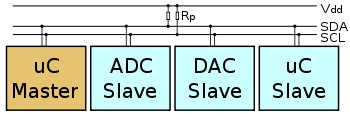
\includegraphics[width=0.3\columnwidth]{img/i2c-bus.png}
% 	\caption{Bus \IIC}%
% 	\label{fig:iic-bus}
% \end{wrapfigure}


% %% %%%%%%%%%%%%%%%%%%%%%%%%%%%%%%%%%%%%%%%%%%%%%%%%%%%%%%%%%%
% intro.tex
%
% Author:  Mauricio Matamoros
% License: MIT
%
% %% %%%%%%%%%%%%%%%%%%%%%%%%%%%%%%%%%%%%%%%%%%%%%%%%%%%%%%%%%%

%!TEX root = ../practica.tex
%!TEX root = ../references.bib

\subsection{MicroPython}%
\label{sec:uPy}

% The use of the Python language for controlling hardware has been around for some time. Users of the Raspberry Pi, pcDuino, and other low-cost computers and similar boards have had the advantage of using Python for controlling hardware. In this case, they used full versions of the Python programming language on the native Linux-based operating system. While these boards made it possible for those who wanted to develop electronics projects, it required users to buy the board as well as peripherals like a keyboard, mouse, and monitor. Not only that, but users also had to learn the operating system. For those not used to Linux, this can be a challenge in and of itself.

% The vision for MicroPython was to combine the simplicity of learning Python with the low cost and ease of use of microcontroller boards, which would permit a lot more people to work with electronics for art and science projects. Beginners would not have to learn a new operating system or learn one of the more complex programming languages.

Creado por Damien P. George y Paul Sokolovsky (entre otros),
MicroPython fue diseñado para ser una versión ligera y eficiente del lenguaje Python 3 instalable en un pequeño microcontrolador.
Dado que Python es un lenguaje interpretado y, por lo tanto, en general más lento que los lenguajes compilados (véase~\Cref{sec:uPy-interpreter}), MicroPython fue diseñado para ser lo más eficiente posible para que pueda ejecutarse en microcontroladores que normalmente son más lentos y tienen mucha menos memoria que una computadora personal típica~\Citep{bell2022MicroPython,bell2022}.

Otro aspecto es que las tarjetas microcontroladores como Arduino requieren que el código sea compilado en otra computadora para producir un código objeto ejecutable que debe ser cargado en dicha tarjeta.
En contraste, dado que MicroPython es un intérprete ejecutándose directamente en el hardware, puede prescindirse del paso intermedio de compilación:
¡se puede ejecutar el código fuente directamente en el hardware!
Esto permite a los fabricantes de hardware construir tarjetas pequeñas y económicas con MicroPython embebido en el chip y que puedan ejecutar virtualmente cualquier programa tanto en la fase de desarrollo como en la de producción~\Citep{bell2022MicroPython,bell2022}.

MicroPython permite crear programas simples, eficientemente especificados y fáciles de entender.
Además, incluye las siguientes características~\Citep{bell2022MicroPython,bell2022}:

\begin{itemize}[nosep]
	\item \textbf{Intérprete interactivo:} MicroPython habilita en la tarjeta física una consola interactiva especial a la que puede acceder conectándose via USB. % CHKTEX 13

	\item \textbf{Bibliotecas estándar de Python:} MicroPython es compatible con muchas de las bibliotecas estándar de Python.
	En general, uno puede confiar en que alrededor del del 80\% de las bibliotecas más utilizadas estarán disponibles.

	\item \textbf{Bibliotecas a nivel de hardware:} MicroPython tiene bibliotecas integradas que le permiten acceder al hardware directamente para encender o apagar pines, leer datos analógicos, leer datos digitales, controlar hardware (PWM) y más.

	\item \textbf{Extensible:} MicroPython también es extensible.
	Ésta es una gran característica para usuarios avanzados que necesitan implementar alguna biblioteca compleja de bajo nivel (en C/C++) e incluir la nueva biblioteca en MicroPython.
\end{itemize}

La mayor limitación de MicroPython  deriva de su facilidad de uso:
aunque MicroPython está altamente optimizado el código se interpreta sobre la marcha lo que agrega una penalización de desempeño y memoria por parte del intérprete.
Esto significa que los proyectos que requieren un alto grado de precisión, un muestreo de datos a alta frecuencia, o comunicaciones a alta velocidad (por ejemplo USB), pueden no ejecutarse lo suficientemente rápido.
Estos problemas suelen superarse con el uso de bibliotecas en C/C++ optimizadas para manejar la comunicación de bajo nivel.
Por otro lado, MicroPython también requiere de un poco más de memoria que el código nativo.
Normalmente, esto no es un problema, aunque debe tomarse en cuenta si el programa va a extenderse con características nuevas.
Los programas más grandes que usan muchas bibliotecas podrían consumir más memoria de la disponible.
Finalmente, como se mencionó anteriormente, MicroPython no implementa todas las funciones de todas las bibliotecas de Python 3~\Citep{bell2022MicroPython,bell2022}.



\subsection{Lenguajes compilados \textsuperscript{v}/\textsubscript{s} lenguajes interpretados}%
\label{sec:uPy-interpreter}
Los lenguajes compilados requieren de un programa externo llamado compilador para convertir el código fuente de una forma legible por humanos a una forma ejecutable binaria que pueda ser entendido y ejecutado con máxima eficiencia por el procesador.
Por otro lado, los lenguajes interpretados no se compilan, sino que se evalúan línea a línea sobre la marcha con un programa llamado intérprete.
Python 3 proporciona un ejecutable de Python que es a la vez un intérprete y una consola que le permite ejecutar el código a medida que se escribe.

Por lo tanto, los lenguajes compilados son mucho más rápidos que los lenguajes interpretados porque el código está preparado (y optimizado) para su ejecución en el microprocesador sin requerir de pasos intermedio en tiempo real para procesar el código antes de la ejecución.

% %% %%%%%%%%%%%%%%%%%%%%%%%%%%%%%%%%%%%%%%%%%%%%%%%%%%%%%%%%%%
% intro-adc.tex
%
% Author:  Mauricio Matamoros
% License: MIT
%
% %% %%%%%%%%%%%%%%%%%%%%%%%%%%%%%%%%%%%%%%%%%%%%%%%%%%%%%%%%%%
% CHKTEX-FILE 1
% CHKTEX-FILE 46
%!TEX root = ../practica.tex
%!TEX root = ../references.bib

\subsection{Convertidor Analógico---Digital}%
\label{sec:intro-adc}
Para leer la señal del LM35 se requiere de un Convertidor Analógico Digital o ADC (por sus siglas en inglés: \emph{Digital-Analog Converter}).
Un ADC se elige con base en dos factores clave: su precisión y su tiempo de muestreo.
Debido a que la aplicación del ADC será convertir mediciones de temperatura y los cambios de temperatura son muy lentos,\footnotemark{} puede obviarse el tiempo de muestreo.
En cuanto a la precisión, los convertidores A/D más comunes son de 8 y 10 bits, de los cuales ha de elegirse uno.

La precisión del ADC se calcula tomando en cuenta el rango de operación y la precisión del componente analógico a discretizar.
El LM35 tiene un rango de \degreesC{205}, una diferencial de voltaje $\Delta{}V=10mV/^{o}C$ y una precisión máxima de \degreesC{0.5}, por lo que el sensor entregará un máximo de 2.5V respecto al voltaje de referencia del mismo, con incrementos de 5mV.
Debido a que 256 valores para un rango de \degreesC{205} en incrementos de \degreesC{0.5} (es decir 410 valores) es claramente insuficiente para este sensor, por lo que será conveniente utilizar un convertidor A/D de 10 bits.

Un ADC típico de 12 bits convertirá las señales analógicas entre voltajes de referencia $V_{Ref-}$ y $V_{Ref+}$ como un entero con valores entre 0 y 4096, interpretando los valores $V_{Ref-}$ como 0 lógico y $V_{Ref+}$ como 4096 de manera aproximadamente lineal.
El decir, la lectura obtenida es directamente proporcional al voltaje dentro del rango, estimable mediante la fórmula:

\begin{equation}
V_{out}= value \times \frac{ V_{Ref+} - V_{Ref-} }{ 4096 }
\end{equation}

En una configuración simple, $V_{Ref-}$ y $V_{Ref+}$ se conectan internamente dentro del RP2040 a tierra y V\textsubscript{CC} respectivamente. Esto simplifica la fórmula como:

\begin{equation}
V_{out}= value \times \frac{ 5V }{ 4096 } = value \times 1.22mV
\end{equation}

En lo concerniente al RP040, éste incorpora un convertidor analógico-digital de 12 bits con soporte para voltaje de referencia $V_{Ref+}$, denominado \emph{ADC\_VREF} según las especificaciones del mismo~\Citep{RP2040datasheet}.
Considerando que el LM35 en rango completo entrega hasta 2.05V ($10mV\times (150 - -55) = 2.05V$) la mayor parte de los 4096 valores jamás serán ocupados.
Por este motivo, conviene sacar partido del pin de voltaje de referencia \emph{ADC\_VREF} del RP2040 mediante un divisor de voltaje (véase~\Cref{fig:lm35-pico}).
En consecuencia, el pin \emph{ADC\_VREF} requerirá de un divisor de voltaje con salida de 2.73V tal como se muestra en la~\Cref{fig:lm35-pico} para dar mayor precisión al convertidor A/D.

\begin{figure}
	\centering
	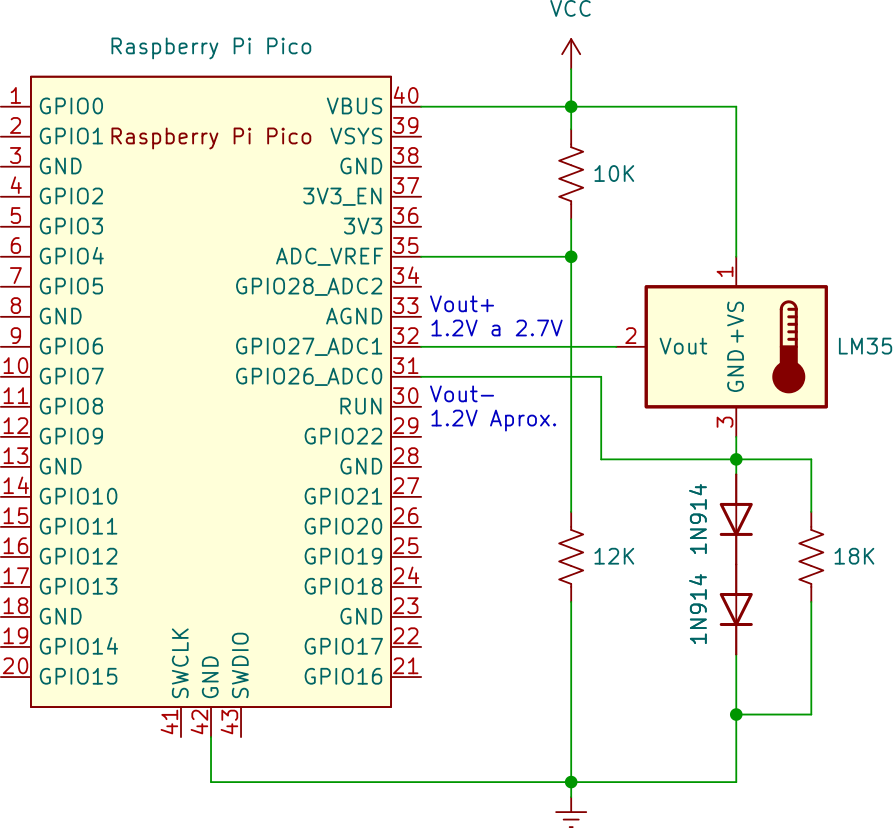
\includegraphics[width=\textwidth,height=7cm,keepaspectratio]{img/lm35-pico.png}
	\caption{Circuito medidor de temperatura LM35 con el RP2040}
	\label{fig:lm35-pico} % chktex 24
\end{figure}

Con esta nueva configuración, se puede calcular de nueva cuenta la precisión del sensor digital una vez decodificado el valor analógico leído del LM35 dividiendo los 2.73V de referencia entre los 4096 valores posibles que entrega el ADC como sigue:

\begin{equation}
\Delta V = \frac{ 2.73V }{ 4096 } =  666.5\times10^{-6}V = 667\mu{}V
\end{equation}

Debido a que la resolución máxima del sensor LM35 determinada por su factor de incertidumbre es de \degreesC{0.5} equivalentes a 0.005V, ambas configuraciones (con y sin el divisor de voltaje) serán adecuadas para operar al sensor.

% %% %%%%%%%%%%%%%%%%%%%%%%%%%%%%%%%%%%%%%%%%%%%%%%%%%%%%%%%%%%
% intro-lm35.tex
%
% Author:  Mauricio Matamoros
% License: MIT
%
% %% %%%%%%%%%%%%%%%%%%%%%%%%%%%%%%%%%%%%%%%%%%%%%%%%%%%%%%%%%%

%!TEX root = ../practica.tex
%!TEX root = ../references.bib


\subsection{Thonny}%
\label{sec:intro-thonny}

Thonny es un IDE\footnote{Entorno de desarrollo integrado, por sus siglas en inglés \emph{Integrated Development Environment}}
de código abierto
para Python desarrollado por la Universidad de Tartu, Estonia, pensado para ser amigable con el principiante.
Además de las capacidades estándar de construcción y ejecución de programas, cuenta con un soporte extendido para animación de programas,
permitiendo ilustrar los conceptos de variables, control de flujo, evaluacíón de expresiones, llamada a funciones, recursión, referencias y montículos, objetos (incluyendo clases y funciones como valores), datos compuestos (listas, diccionarios y conjuntos) y operaciones de entrada/salida sobre archivos~\Citep{annamaa2015a,annamaa2015b}.

Thonny puede llevar registro de las acciones del usuario con suficiente detalle para reproducir el proceso de elaboración de un programa, permitiéndole a los estudiantes elegir el nivel de detalle con el que desean analizar la reproducción~\Citep{annamaa2015a,annamaa2015b}.

Una de las ventajas de Thonny sobre cualquier otro editor de Python es que, a partir de la versión 4.0, incluye soporte para interactuar con varios  microcontroladores como el RP2040, el ESP32 y el ESP8266; todos de amplia difusión en el mercado.
Además, Thonny permite realizar operaciones en el sistema de archivos virtual del RP2040 (MicroPython convierte el RP2040 en una suerte de memoria USB de unos cuantos kB).
Para este fin, basta con contectar la tarjeta controladora a la PC, iniciar Thonny y seleccionar las opciones \emph{View} y \emph{Files}.
De igual manera Thony permite copiar archivos de y a la tarjeta controladora para ser utilizados por MicroPython~\cite{bell2022MicroPython,bell2022}.

\begin{figure}[H]
	\centering%
	\includegraphics[width=\columnwidth,height=8cm,keepaspectratio]{img/thonny-files.png} %CHKTEX 8
	\caption{Thonny permite visualizar, crear, copiar, cortar, pegar y, en general, manupular archivos dentro del RP2040.}
	\label{fig:thonny} %CHKTEX 24
\end{figure}


% CHKTEX-FILE 1
% CHKTEX-FILE 13
% CHKTEX-FILE 46
%!TEX root = ../practica.tex
%!TEX root = ../references.bib

%% %%%%%%%%%%%%%%%%%%%%%%%%%%%%%%%%%%%%%%%%%%%%%%%%%%%%%%%%%%%%%%%%%%
%
% Material
%
%% %%%%%%%%%%%%%%%%%%%%%%%%%%%%%%%%%%%%%%%%%%%%%%%%%%%%%%%%%%%%%%%%%%
\section{Material}%
\label{sec:material}
Se asume que el alumno cuenta con un una Raspberry Pi con sistema operativo Raspbian e interprete de Python instalado. Se aconseja encarecidamente el uso de \textit{git} como programa de control de versiones.

\begin{itemize}[noitemsep]
	\item 1 microcontrolador RP2040 (ej. Raspnerry Pi Pico) con MicroPython precargado.
	\item 1 TRIAC BT138 o BT139
	\item 4 diodos 1N4007 o puente rectificador equivalente
	\item 1 optoacoplador MOC 3021
	\item 1 optoacoplador 4N25
	\item 1 foco incandescente (NO AHORRADOR NI LED)
	\item 1 resistencia de 68k$\Omega$, \sfrac{1}{4}Watt
	\item 1 resistencia de 10k$\Omega$, \sfrac{1}{4}Watt
	\item 2 resistencia de 4k7$\Omega$, \sfrac{1}{4}Watt
	\item 1 resistencia de  1k$\Omega$, 1Watt
	\item 2 resistencia de 470$\Omega$, \sfrac{1}{4}Watt
	\item 2 resistencia de 330$\Omega$, \sfrac{1}{4}Watt
	\item 1 LED de 5mm
	\item 1 LED ultrabrillante de 5mm
	\item 1 protoboard o circuito impreso equivalente
	\item 1 fuente de alimentación regulada a 5V y al menos 2 amperios de salida
	\item Cables y conectores varios
\end{itemize}

% %% %%%%%%%%%%%%%%%%%%%%%%%%%%%%%%%%%%%%%%%%%%%%%%%%%%%%%%%%%%
% steps.tex
%
% Author:  Mauricio Matamoros
% License: MIT
%
% %% %%%%%%%%%%%%%%%%%%%%%%%%%%%%%%%%%%%%%%%%%%%%%%%%%%%%%%%%%%

%!TEX root = ../practica.tex
%!TEX root = ../references.bib

\section{Instrucciones}%
\label{sec:instructions}
\begin{enumerate}[noitemsep]
	\item Alambre el circuito mostrado en la \Cref{fig:lm35-pico}.
	\item Realice los programas de las \Cref{sec:step3,sec:step4}
 	\item Analice los programas de las \cref{sec:step3,sec:step4}, realice los experimentos propuestos en la \cref{sec:experiments}.
 	% y con los resultados obtenidos responda el cuestionario de la \cref{sec:questionnaire}.
\end{enumerate}

% %% %%%%%%%%%%%%%%%%%%%%%%%%%%%%%%%%%%%%%%%%%%%%%%%%%%%%%%%%%%
% step-1.tex
%
% Author:  Mauricio Matamoros
% License: MIT
%
% %% %%%%%%%%%%%%%%%%%%%%%%%%%%%%%%%%%%%%%%%%%%%%%%%%%%%%%%%%%%

%!TEX root = ../practica.tex
%!TEX root = ../references.bib

% CHKTEX-FILE 1
% CHKTEX-FILE 13
% CHKTEX-FILE 46

\subsection{Paso 1: Descargar MicroPython}%
\label{sec:step1}

Ingrese a \url{https://micropython.org/download/?port=rp2} y seleccione el modelo de su tarjeta controladora.
Si no está seguro, simplemente de click en la imagen correspondiente a la Raspberry Pi Pico (\url{https://micropython.org/download/rp2-pico/}).
A continuación descargue último firmware disponible de MicroPython, por ejemplo la \href{https://micropython.org/resources/firmware/rp2-pico-20230426-v1.20.0.uf2}{versión 1.20.0}.
Deberá ser un archivo extensión \code{uf2}.

\begin{figure}[H]
	\centering%
	\begin{subfigure}[b]{0.45\textwidth}
		\centering%
		\includegraphics[width=\columnwidth,height=8cm,keepaspectratio]{img/upy-dl-01.png} %CHKTEX 8
		\caption{Selección de la Raspberry Pi Pico}
		\label{fig:upy-dl-a} %CHKTEX 24
	\end{subfigure}
	\hfill
	\begin{subfigure}[b]{0.45\textwidth}
		\centering%
		\includegraphics[width=\columnwidth,height=8cm,keepaspectratio]{img/upy-dl-02.png} %CHKTEX 8
		\caption{Firmwares disponibles}
		\label{fig:upy-dl-b} %CHKTEX 24
	\end{subfigure}
	\caption{Descarga de la última versión de MicroPython}
	\label{fig:upy-dl} %CHKTEX 24
\end{figure}

\begin{greenbox}{Importante}
	Si tiene una Raspberry Pi Pico-W descargue el firmware para la Pico-W.
	De otro modo no podrá usar la tarjeta inalámbrica
\end{greenbox}


% %% %%%%%%%%%%%%%%%%%%%%%%%%%%%%%%%%%%%%%%%%%%%%%%%%%%%%%%%%%%
% step-2.tex
%
% Author:  Mauricio Matamoros
% License: MIT
%
% %% %%%%%%%%%%%%%%%%%%%%%%%%%%%%%%%%%%%%%%%%%%%%%%%%%%%%%%%%%%

%!TEX root = ../main.tex
%!TEX root = ../references.bib

\subsection{Paso 2: Led parpadeante}%
\label{sec:step2}
El código mostrado en \Cref{src:blink} muestra cómo se haría parpadear un LED mediante tiempos de espera o \emph{sleeps} utilizando la Raspberry Pi.

\smallskip
\lstinputlisting[%
	language=Python,
	linerange={18-40}, % chktex 8
	caption={\texttt{blink.py}},
	label={src:blink}
]{src/blink.py}
\smallskip

Estudie el código y véalo en funcionamiento, ejecutándolo de la siguiente manera:
\begin{Verbatim}[fontsize=\footnotesize]
./blink.py
\end{Verbatim}

% %% %%%%%%%%%%%%%%%%%%%%%%%%%%%%%%%%%%%%%%%%%%%%%%%%%%%%%%%%%%
% step-3.tex
%
% Author:  Mauricio Matamoros
% License: MIT
%
% %% %%%%%%%%%%%%%%%%%%%%%%%%%%%%%%%%%%%%%%%%%%%%%%%%%%%%%%%%%%

%!TEX root = ../practica.tex
%!TEX root = ../references.bib

% CHKTEX-FILE 1
% CHKTEX-FILE 13
% CHKTEX-FILE 46

\subsection{Paso 3: Configuración de comunicaciones \IIC}%
\label{sec:step3}
Primero ha de configurarse la Raspberry Pi para funcionar como dispositivo maestro o \emph{master} en el bus \IIC.
Para esto, inicie la utilidad de configuración de la Raspberry Pi con el comando

\begin{Verbatim}
# raspi-config
\end{Verbatim}

\noindent y seleccione la opción 5: Opciones de Interfaz (\emph{Interfacing Options}) y active la opción \texttt{P5} para habilitar el \IIC.

A continuación, verifique que el puerto \IIC no se encuentre en la lista negra.
Edite el archivo \\\texttt{/etc/modprobe.d/raspi-blacklist.conf} y revise que la línea \texttt{blacklist spi-bcm2708} esté comentada con \#.

% $ cat /etc/modprobe.d/raspi-blacklist.conf
\begin{lstlisting}[
	language=conf,
	caption={/etc/modprobe.d/raspi-blacklist.conf},
	label={lst:raspi-blacklist.conf},
	numbers=none
]
# blacklist spi and i2c by default (many users don't need them)
# blacklist i2c-bcm2708
\end{lstlisting}

Como paso siguiente, se habilita la carga del driver \IIC.
Esto se logra agregando la línea \texttt{i2c-dev} al final del archivo \texttt{/etc/modules} si esta no se encuentra ya allí.

Por último, se instalan los paquetes que permiten la comunicación mediante el bus \IIC y se habilita al usuario predeterminado \emph{pi} (o cualquier otro que se esté usando) para acceder al recurso.

\begin{Verbatim}
# apt-get install i2c-tools python3-smbus
# adduser pi i2c
$ pip install smbus2
\end{Verbatim}

Reinicie la Raspberry Pi y pruebe la configuración ejecutando \texttt{i2cdetect -y 1} para buscar dispositivos conectados al bus \IIC.
Debería ver una salida como la siguiente:

% CHKTEX-FILE 8
\begin{Verbatim}
$ i2cdetect -y 1
     0  1  2  3  4  5  6  7  8  9  a  b  c  d  e  f
00:          -- -- -- -- -- -- -- -- -- -- -- -- --
10: -- -- -- -- -- -- -- -- -- -- -- -- -- -- -- --
20: -- -- -- -- -- -- -- -- -- -- -- -- -- -- -- --
30: -- -- -- -- -- -- -- -- -- -- -- -- -- -- -- --
40: -- -- -- -- -- -- -- -- -- -- -- -- -- -- -- --
50: -- -- -- -- -- -- -- -- -- -- -- -- -- -- -- --
60: -- -- -- -- -- -- -- -- -- -- -- -- -- -- -- --
70: -- -- -- -- -- -- -- --
\end{Verbatim}

% %% %%%%%%%%%%%%%%%%%%%%%%%%%%%%%%%%%%%%%%%%%%%%%%%%%%%%%%%%%%
% step-4.tex
%
% Author:  Mauricio Matamoros
% License: MIT
%
% %% %%%%%%%%%%%%%%%%%%%%%%%%%%%%%%%%%%%%%%%%%%%%%%%%%%%%%%%%%%

%!TEX root = ../practica.tex
%!TEX root = ../references.bib

% CHKTEX-FILE 1
% CHKTEX-FILE 13
% CHKTEX-FILE 46

\subsection{Paso 4: Configuración del \emph{root filesystem}}%
\label{sec:step4}
El siguiente paso consiste en configurar el sistema de archivos raíz o \emph{root filesystem}.
Tras compilar el kernel y los paquetes solicitados, \emph{buildroot} tomará el directorio especificado y sobrepondrá el contenido de éste al sistema de archivos raíz que está siendo generado, un proceso conocido como superposición u \emph{overlay}.

El directorio de superposición puede ser cualquiera en el disco duro.
Sin embargo, se estila colocarlo como un subdirectorio de nombre \texttt{rootfs-overlay} dentro de \texttt{board/<company>/<boardname>}
que, si inspecciona con \texttt{ls}, notará que contiene ya varios archivos de configuración para nuestra tarjeta Raspberry Pi 4 de 64bits.
En nuestro caso la ruta relativa será:

\begin{Verbatim}[gobble=1]
	board/raspberrypi4-64/rootfs-overlay
\end{Verbatim}

Es en este directorio donde colocaremos todos los archivos y directorios que querramos contenga la imagen generada.

Ejecute los siguientes comando para crear el directorio \emph{home} del usuario \emph{pi} creado en el paso anterior y otros directorios que serán necesarios para configuar al sistema embebido.

\begin{Verbatim}[gobble=1]
	mkdir -p board/raspberrypi4-64/rootfs-overlay/home/pi
	mkdir -p board/raspberrypi4-64/rootfs-overlay/etc/init.d
\end{Verbatim}

El sistema creado por \emph{buildroot} es un sistema mínimo.
Esto quiere decir que no se incluye nada que no sea indispensable a menos que sea declarado de forma explícita,
y esto se logra añadiendo los archivos de configuración pertinente al sistema de archivos raíz o \emph{root filesystem} (en adelante rootFS).
Por ejemplo, los controladores para \IIC{} no se cargan de forma predeterminada.

Para especificar el rootFS en \emph{buildroot} ejecute \texttt{make menuconfig} y localice la opción \emph{root filesystem overlay directories} bajo el menú de configuración del sistema (\emph{system configuration}) con el valor del directorio creado anteriormente, es decir:

\begin{Verbatim}[gobble=1]
	board/raspberrypi4-64/rootfs-overlay
\end{Verbatim}

Para indicarle al kernel que debe cargar los controladores para \IIC{} haremos uso de dos archivos.
El primero será el archivo \texttt{S02modules} localizado en \texttt{etc/init.d}, directorio que contiene todos los scripts de arranque del sistema y que son ejecutados en orden.%
\footnote{
	Los controladores tienen muy alta prioridad, de allí que se tengan que cargar primero que otros servicios.
	Es por esto que el nombre del archivo comienza con S02, y será ejecutado después de todos los S00 y S01.
}
\begin{samepage}
Procedemos a crear el archivo, marcarlo como ejecutable y editarlo con los siguientes dos comandos:

\begin{Verbatim}[gobble=1]
	touch board/raspberrypi4-64/rootfs-overlay/etc/init.d/S02modules
	chmod +x board/raspberrypi4-64/rootfs-overlay/etc/init.d/S02modules
	nano board/raspberrypi4-64/rootfs-overlay/etc/init.d/S02modules
\end{Verbatim}
\end{samepage}

\medskip{}

\begin{importantbox}{Advertencia}
	Los archivos que está a punto de modificar son relativos al directorio de la tarjeta dentro de buildroot.

	\medskip\bfseries
	Por ningún motivo modifique los archivos en el directorio \texttt{/etc} de su sistema anfitrión.
\end{importantbox}

\medskip{}
% \newpage

\begin{samepage}
\noindent
A coninuación, agregue el siguiente contenido al archivo:

\noindent
\begin{minipage}{\columnwidth}
\begin{lstlisting}[%
	title={\texttt{rootfs-overlay/etc/init.d/S02modules}},%
	firstnumber=1]
#!/bin/sh
case "${1}" in
    start)
        # Exits if /etc/modules does not exists or lacks valid entries
        [ -r /etc/modules ] && egrep -qv '^($|#)' /etc/modules || exit 0
        # Load listed modules
        while read module args; do
            # Skip comments and empty lines.
            case "$module" in
                ""|"#"*) continue ;;
            esac
            # Try to load each module
            printf "Loading ${module}"
            modprobe ${module} ${args} > /dev/null
            [ $? = 0 ] && echo "OK" || echo "FAIL"
        done < /etc/modules
        exit 0
        ;;

    *)
        echo "Usage: ${0} {start}"
        exit 1
        ;;
esac
\end{lstlisting}
\end{minipage}
\end{samepage}

\texttt{S02modules} es un script de carga de controladores (módulos) simple y genérico que cargará de forma dinámica todos los controladores listados en otro archivo llamado \texttt{modules} en el directorio \texttt{/etc}, si existe.
Procedamos pues a crear dicho archivo con un editor de texto como \texttt{nano}.

\begin{Verbatim}[gobble=1]
	nano board/raspberrypi4-64/rootfs-overlay/etc/modules
\end{Verbatim}

\begin{samepage}
\noindent
A coninuación, agregue el siguiente contenido al archivo:

\noindent
\begin{minipage}{\columnwidth}
\begin{lstlisting}[%
	title={\texttt{rootfs-overlay/etc/modules}},%
	firstnumber=1]
# List of modules to be loaded during startup
i2c-bcm2835
i2c-dev
\end{lstlisting}
\end{minipage}
\end{samepage}

Estos archivos harán que el kernel cargue los controladores para \IIC{} al arranque, ¡pero \texttt{/dev/i2c-1} sólo será accesible por el superusuario \emph{root}!
Para solucionar este inconveniente crearemos otro script de arranque similar a \texttt{S02modules} que cambie los permisos de todos los periféricos \IIC{} cambiando su grupo a i2c al cual el usuario \emph{pi} que creamos en el paso anterior ya tiene acceso.

\begin{samepage}
Procedemos a crear el archivo, marcarlo como ejecutable y editarlo con los siguientes dos comandos:

\begin{Verbatim}[gobble=1]
	touch board/raspberrypi4-64/rootfs-overlay/etc/init.d/S10i2cperms
	chmod +x board/raspberrypi4-64/rootfs-overlay/etc/init.d/S10i2cperms
	nano board/raspberrypi4-64/rootfs-overlay/etc/init.d/S10i2cperms
\end{Verbatim}
\end{samepage}

\begin{samepage}
\noindent
A continuación, agregue el siguiente contenido al archivo:

\noindent
\begin{minipage}{\columnwidth}
\begin{lstlisting}[%
	title={\texttt{rootfs-overlay/etc/init.d/S10i2cperms}},%
	firstnumber=1]
#!/bin/sh
case "${1}" in
    start)
        # Loops over all i2c devices, if any
        for iic in /dev/i2c*; do
            chown root:i2c "${iic}"
            chmod ug+rw "${iic}"
        done
        unset iic
        ;;

    *)
        echo "Usage: ${0} {start}"
        exit 1
        ;;
esac
\end{lstlisting}
\end{minipage}
\end{samepage}

\medskip{}

Por último, crearemos los archivos que permitan la ejecución automática de cualquer script de arranque que nos sea conveniente:

\begin{enumerate}
	\item Copie el archivo anexo \texttt{test.pyc} al directorio del usuario \emph{pi}; es decir a\\
	\texttt{board/raspberrypi4-64/rootfs-overlay/home/pi}.

	\begin{samepage}
	\item Cree un archivo de inicio \texttt{start.sh} en el mismo directorio, y márquelo como ejecutable con los siguientes comandos:
	\begin{Verbatim}[gobble=2]
		touch board/raspberrypi4-64/rootfs-overlay/home/pi/start.sh
		chmod +x board/raspberrypi4-64/rootfs-overlay/home/pi/start.sh
	\end{Verbatim}
	\end{samepage}

	\begin{samepage}
	\item Utilizando editor de texto plano como \texttt{nano} o \texttt{vim}, edite el archivo anterior y agregue el siguiente contenido al archivo:
	\lstinputlisting[%
		language=sh,%
		title={\texttt{rootfs-overlay/home/pi/start.sh}},%
		linerange={1-43}%
	]{src/board/raspberrypi4-64/rootfs-overlay/home/pi/start.sh}
	\end{samepage}

	\begin{samepage}
	\item Cree un archivo de autoarranque o \emph{daemon} \texttt{S99autostart} en el mismo directorio \texttt{etc/init.d/} del \emph{overlay}, y márquelo como ejecutable con los siguientes dos comandos:
	\begin{Verbatim}[gobble=2]
		touch board/raspberrypi4-64/rootfs-overlay/etc/init.d/S99autostart
		chmod +x board/raspberrypi4-64/rootfs-overlay/etc/init.d/S99autostart
	\end{Verbatim}
	\end{samepage}

	\begin{samepage}
	\item Utilizando editor de texto plano como \texttt{nano} o \texttt{vim}, edite el archivo \texttt{S99autostart} y agregue el siguiente contenido al archivo:\\
\noindent
\begin{minipage}{\columnwidth}
\begin{lstlisting}[%
	title={\texttt{rootfs-overlay/etc/init.d/S99autostart}},%
	firstnumber=1]
#!/bin/sh
case "${1}" in
    start)
        # Exits if /home/pi/start.sh does not exist
        [ -f /home/pi/start.sh ] || exit 0
        # Else executes it
        su - pi -c /home/pi/start.sh
        exit 0
        ;;

    *)
        echo "Usage: ${0} {start}"
        exit 1
        ;;
esac
\end{lstlisting}
\end{minipage}
\end{samepage}

\end{enumerate}

\noindent
¡Listo! Ahora su sistema puede ejecutar programas como el usuario \emph{pi} automáticamente al arrancar.
Sólo tiene que modidificar el archivo \texttt{home/pi/start.sh} de acuerdo a sus necesidades.

\bigskip{}

Opcionalmente, en caso de que se haya llevado a cabo la personalización con logotipo~(véase~\Cref{sec:step3}), procederemos a automatizar la solución del inconveniente y borrar la pantalla de forma automática cuando se inicie sesión.
Esto se logra de forma simple añadiendo dicho comando al final del archivo \texttt{.profile} ubicado en cada uno de los directorios de usuario, en nuestro caso \texttt{/root} y \texttt{/home/pi}.

\begin{samepage}
Para resolver el inconveniente el caso del súperusuario \emph{root} ejecute los siguientes comandos:
\begin{Verbatim}[gobble=1]
	$ mkdir -p board/raspberrypi/rootfs-overlay/root
	$ echo "clear" > board/raspberrypi/rootfs-overlay/root/.profile
\end{Verbatim}
\end{samepage}

\begin{samepage}
A continuación, repetimos el procedimiento para la cuenta de usuario \emph{pi}:

\begin{Verbatim}[gobble=1]
	$ echo "clear" > board/raspberrypi/rootfs-overlay/home/pi/.profile
\end{Verbatim}
\end{samepage}

Listo.
Hemos terminado de configurar el sistema de archivos.


% %% %%%%%%%%%%%%%%%%%%%%%%%%%%%%%%%%%%%%%%%%%%%%%%%%%%%%%%%%%%
% experiments.tex
%
% Author:  Mauricio Matamoros
% License: MIT
%
% %% %%%%%%%%%%%%%%%%%%%%%%%%%%%%%%%%%%%%%%%%%%%%%%%%%%%%%%%%%%
%!TEX root = ../practica.tex
%!TEX root = ../references.bib

% CHKTEX-FILE 1
% CHKTEX-FILE 13
% CHKTEX-FILE 46

\section{Experimentos}%
\label{sec:experiments}

\begin{enumerate}
	\item{} [6pt] Alambre el circuito completo y combine el código de los \Cref{sec:appendix1,sec:appendix2,sec:appendix3} para poder controlar la intensidad del brillo del foco incandecente con la Raspberry Pi usando los valores tecleados en la consola (porentaje de 0--100\% de la potencia total).

	\item{} [4pt] Modifique el código anterior para que la consola presente la potencia real modulada por el Arduino (equivalente en potencia del tiempo de encendido en milisegundos).

	% \item{} [+3pt] Modifique el código del punto 2 para que el arduino pueda modular la potencia del foco incandecente entre 0\% y 100\% con una resolución máxima de 1\%. Imprima la potencia reportada por el arduino con un dígito decimal.
	% Justifique el código modificado con los cálculos pertinentes que prueben que los valores reportados son correctos dentro de la resolución solicitada.

	\item{} [+2pt] Con base en lo aprendido, modifique el código delpunto 3 para que la Raspberry Pi sirva una página web donde se pueda modificar con un control gráfico la potencia de encendido del foco.
\end{enumerate}

% %% %%%%%%%%%%%%%%%%%%%%%%%%%%%%%%%%%%%%%%%%%%%%%%%%%%%%%%%%%%
% references.tex
%
% Author:  Mauricio Matamoros
% License: MIT
%
% %% %%%%%%%%%%%%%%%%%%%%%%%%%%%%%%%%%%%%%%%%%%%%%%%%%%%%%%%%%%
%!TEX root = ../practica.tex
%!TEX root = ../references.bib

% CHKTEX-FILE 1
% CHKTEX-FILE 13
% CHKTEX-FILE 46

\cleardoublepage
% \section{Referencias}%
% \label{sec:references}
\nocite{*}
\bibliographystyle{unsrtnat}
\bibliography{references}


\appendix

% % %% %%%%%%%%%%%%%%%%%%%%%%%%%%%%%%%%%%%%%%%%%%%%%%%%%%%%%%%%%%
% apendices.tex
%
% Author:  Mauricio Matamoros
% License: MIT
%
% %% %%%%%%%%%%%%%%%%%%%%%%%%%%%%%%%%%%%%%%%%%%%%%%%%%%%%%%%%%%

%!TEX root = ../practica.tex
%!TEX root = ../references.bib

\cleardoublepage{}
\section{Programa Ejemplo: \texttt{blink.py}}%
\label{sec:appendix1}
\lstinputlisting[language=python,firstline=11]%
{src/blink.py}

% \cleardoublepage{}
\section{Programa Ejemplo: \texttt{blink-timer.py}}%
\label{sec:appendix2}
\lstinputlisting[language=Python,firstline=11]%
{src/blink-timer.py}

% \cleardoublepage{}
\section{Programa Ejemplo: \texttt{temp.py}}%
\label{sec:appendix3}
\lstinputlisting[language=Python,firstline=11]%
{src/temp.py}


\end{document}
